\documentclass[12pt]{article}
\usepackage[a4paper, margin=1in]{geometry}

\usepackage{hyperref}
\usepackage{amsfonts, amsmath, amssymb, amsthm}
\usepackage{graphicx}
\usepackage{subfigure}
\usepackage{caption}
\usepackage{subcaption}
\usepackage{fancyhdr}



\begin{document}
	\begin{titlepage}
		\begin{center}
			\begin{figure}
				\centering
				
\includegraphics[scale=0.15]{images/IUST_Logo.jpg} \\
				\caption*{\textbf{School of Mathematics \& Computer Science}}
			\end{figure}
			\vspace*{0.5cm}
			\Huge{\textbf{Comparison of \\ Numerical Methods and PINNs \\ for the Schrödinger equation}}\\
			\vspace*{3cm}
			\large{\textbf{Mohsen Peykanro}}\\
			\large{\textbf{Ehsan Pichka}}\\
			\large{\textbf{Arshia Soleymani}}\\
			\vspace*{3cm}
			\large{\textbf{Advisor:}}\\
			\large{\textbf{Dr. Mahboubeh Molavi Arabshahi}}\\
			\vspace*{3cm}
			\today
		\end{center}
	\end{titlepage}
	
\section{Introduction}
\subsection{Background}
The Schrödinger equation is a partial differential equation in quantum mechanics that describes how the quantum state of a physical system change over time. This equation can handle the behavior of particles at the microscopic level. This equation have two forms that are based on times. The time-dependent Schrödinger equation describes the change of a system's wave function over time, while the time-independent version is used to determine stationary states and energy levels.

In most cases, you cant solve the equation so the exact analytical solutions are not available, especially for complex potentials or higher-dimensional systems. As a result, numerical methods play a crucial role in approximating solutions. The solution to the Schrödinger equation is called the wave function that provides information about the probability distribution of a particle's position and momentum. We mostly are going to survey Classical numerical approaches and Physics-Informed Neural Networks (PINNs) in this article.

The Classical numerical approaches such as the finite difference method (FDM) and finite element method (FEM) have been widely used for solving partial differential equations like Schrödinger equation. These methods rely on discretization of the domain and typically require careful handling of stability, convergence, and computational cost. On the other hand in recent years, PINNs have appeard as a modern approach for solving differential equations. PINNs merge the physical laws directly into the loss function of a neural network, so the solution will be approximated without discretization of the domain. This makes PINNs usefull for complex and high-dimensional problems.

\subsection{Objective of the Study}
The main objective of this paper is to compare classical numerical methods and Physics-Informed Neural Networks in solving the Schrödinger equation. Despite the growing interest in PINNs, we are not quite sure that how they compare to classical numerical methods in terms of accuracy, efficiency, and stability. A systematic comparison is necessary to evaluate their strengths and limitations.

\section{Mathematical Formulation}
\subsection{Early-Stage Quantum Theory}
The Schrödinger equation is a direct consequence of the discovery of quanta in the early 20th century. Its origins lie in the energy quanta hypothesis proposed by Max Planck in 1900 and the photon hypothesis by Albert Einstein in 1905, which established that energy and momentum are quantized.
\begin{equation}  \label{eq:1905}
	E = h \nu = \hbar \omega
\end{equation} 
where $E$ denotes energy, $h$ is the Plnack constant ($6.626 \times 10^{-34} \,\text{J·s}$) and $\nu$ is frequency of light. so now we can define the reduced Planck constant as $\hbar = \frac{h}{2 \pi}$ and $\omega = 2 \pi \nu$ as angular frequency. 
Later on, Einstein in 1917 concluded that momentum of light quantum $p$ is:
\begin{equation}  \label{eq:1917}
	 p = \frac{E}{c} = \frac{\hbar \omega}{c} = \hbar k 
\end{equation}
$k$ is called wavenumber and is defind as $ k = 2 \pi \lambda$, where $\lambda$ is wavelength of light in vacuum.

In 1923, Arthur Compton conducted experiments investigating how incident X-ray beams were scattered by matter, such as graphite and copper. He discovered a systematic redshift (an increase in wavelength) in the scattered X-rays and they call it Compton effect. Moreover he found that the shift in wavelengths depended only on the scattering angle regardless of quality of material of a scatterer. 
\begin{equation}
	\Delta \lambda = \frac{h}{m_e c} (1 - \cos \theta) 
\end{equation} 
where $\Delta \lambda$ means a Shift in wave length of scatterd beam, $m_e$ is a rest mass of an electron (mass that is independent of the motion of the particle) and $\theta$ is a scatering angle of the beam. The constant $\frac{h}{m_e c} $ is defined as the electron Compton wavelength ( $\lambda_e$) approximately $ 2.426 \times 10^{-12} $ meters.

In 1924, Louis de Broglie Encouraged by the success of Einstein and Compton in proving that waves (light) could behave like particles and theorized that the reverse must also be true, in other word matter particles must possess a wave nature. De Broglie essentially reversed the relationship of (\ref{eq:1905}) and (\ref{eq:1917}) such that
\begin{equation}
	\omega = \frac{E}{\hbar}, \quad k = \frac{p}{\hbar} \quad \text{or} \quad \lambda = \frac{h}{p}
\end{equation}
where $p$ equals $|p|$ and $\lambda$ is a wavelength of a corpuscular beam(a directional stream of tiny particles). this is called de Broglie wavelength (matter wave). this equation implies that if we are able to determine the wavelength of the corpuscular beam experimentally, we can decide a magnitude of momentum accordingly.

For a matter wave, the phase velocity $v_p$ is shown to be greater than $c$, while the group velocity $v_g$, which represents the propagation velocity of a wave packet (and thus the particle's velocity), is less than $c$. Their relationship is defined by $v_p v_g = c^2$. Therefore, a particle velocity must not exceed $c$.
\begin{figure}[h!]
	\centering
	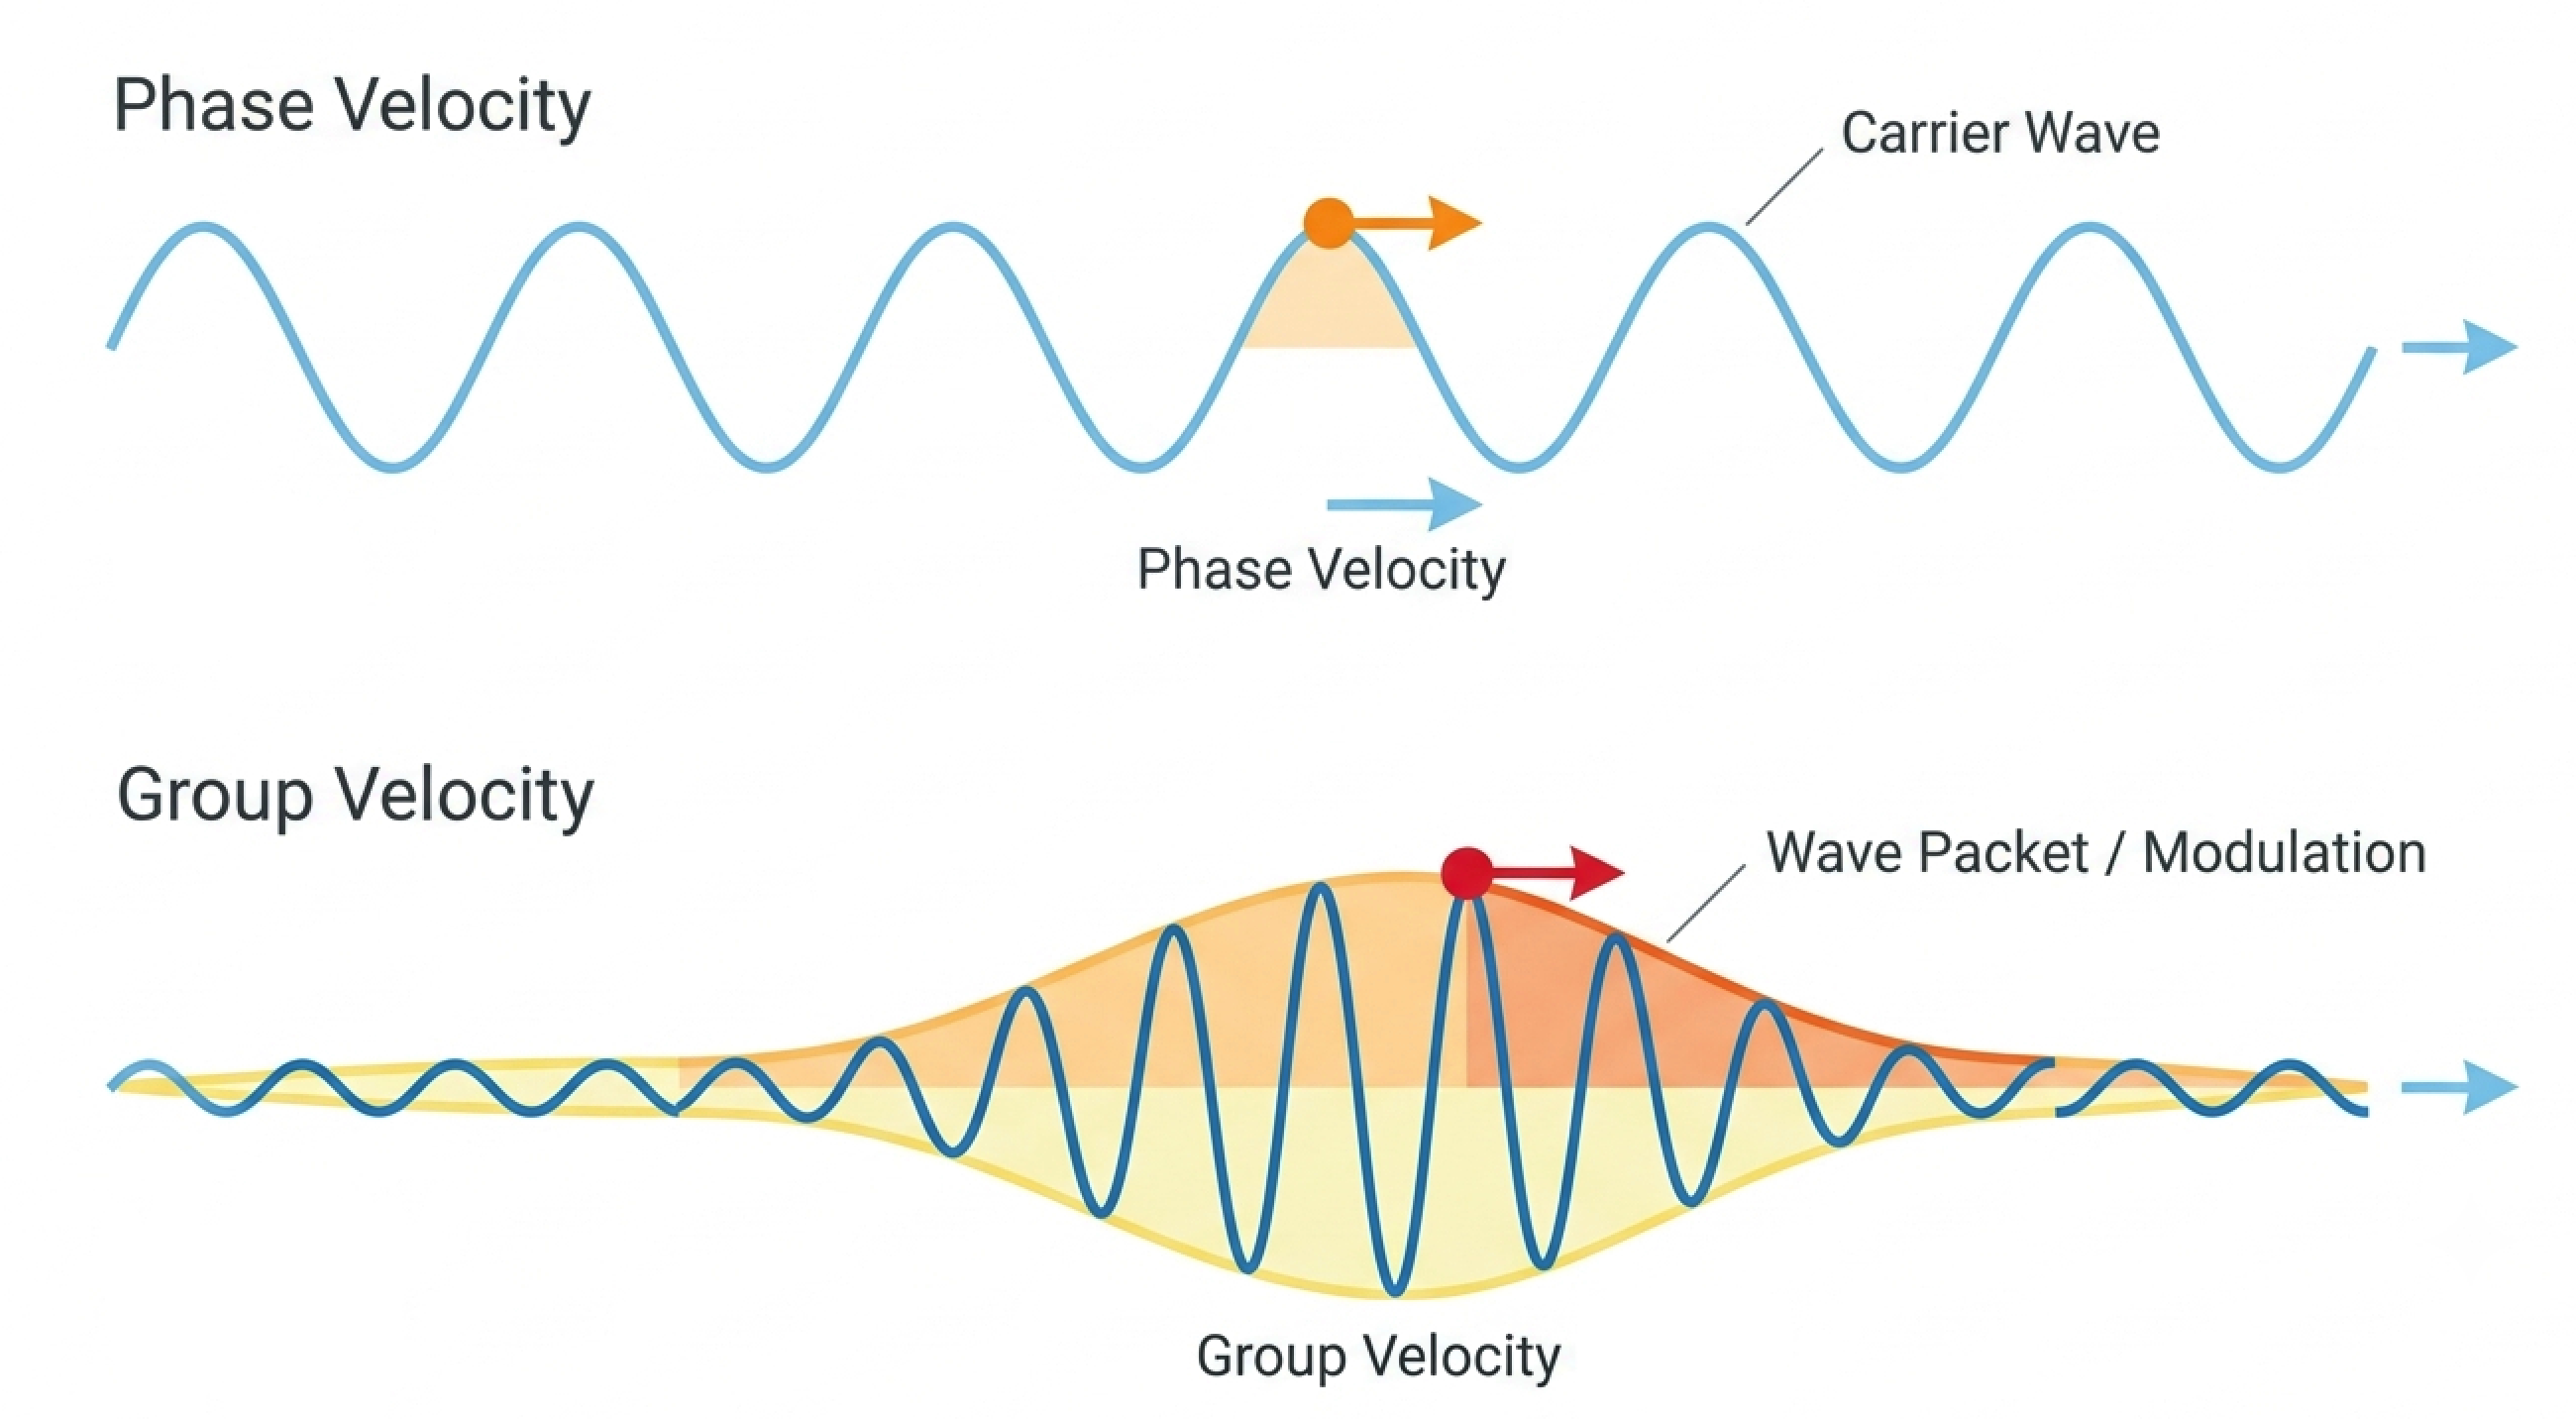
\includegraphics[height=6cm]{images/Fig2}
	\caption{Phase velocity vs Group velocity}
\end{figure}

\subsection{Schrödinger Equation}
The derivation starts with the standard wave equation 
\begin{equation}
	\nabla^2 \Psi = \frac{1}{v^2} \frac{\partial^2 \Psi}{\partial t^2}
\end{equation}
where $\Psi$ is an arbitrary function of a physical quantity relevant to propagation of a wave(shape of a wave), $v$ is a phase velocity of wave, $ \nabla^2$ is called Laplacian and is defined as
\begin{equation}
	\nabla^2 \equiv \frac{\partial^2}{\partial x^2} + \frac{\partial^2}{\partial y^2} + \frac{\partial^2}{\partial z^2}
\end{equation}

\begin{figure}[h!]
	\centering
	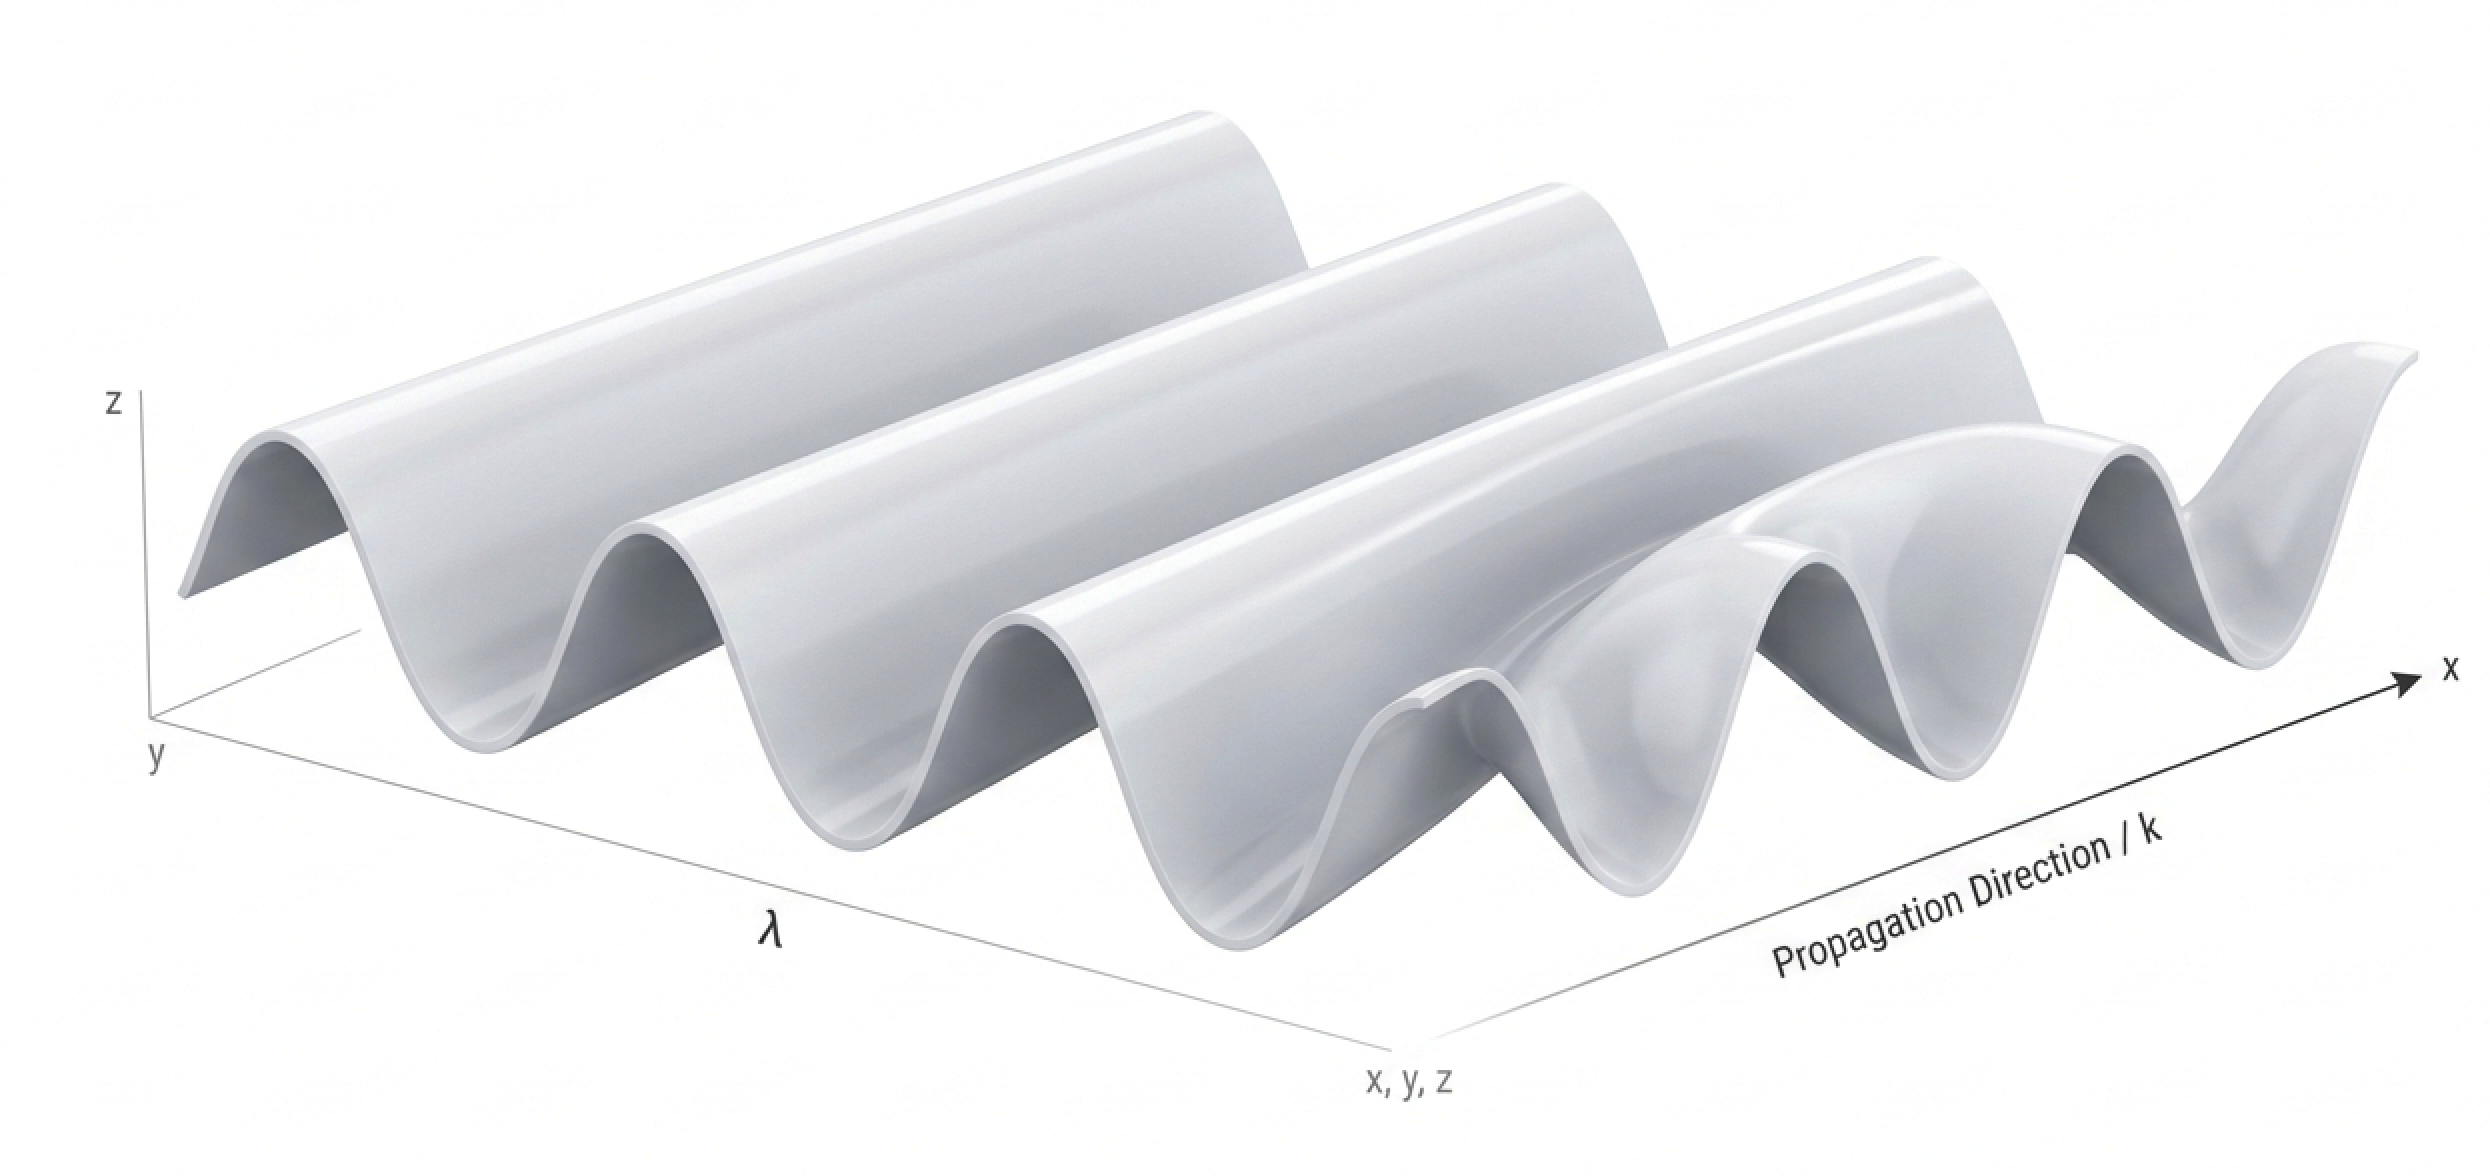
\includegraphics[width=7cm]{images/Fig3}
	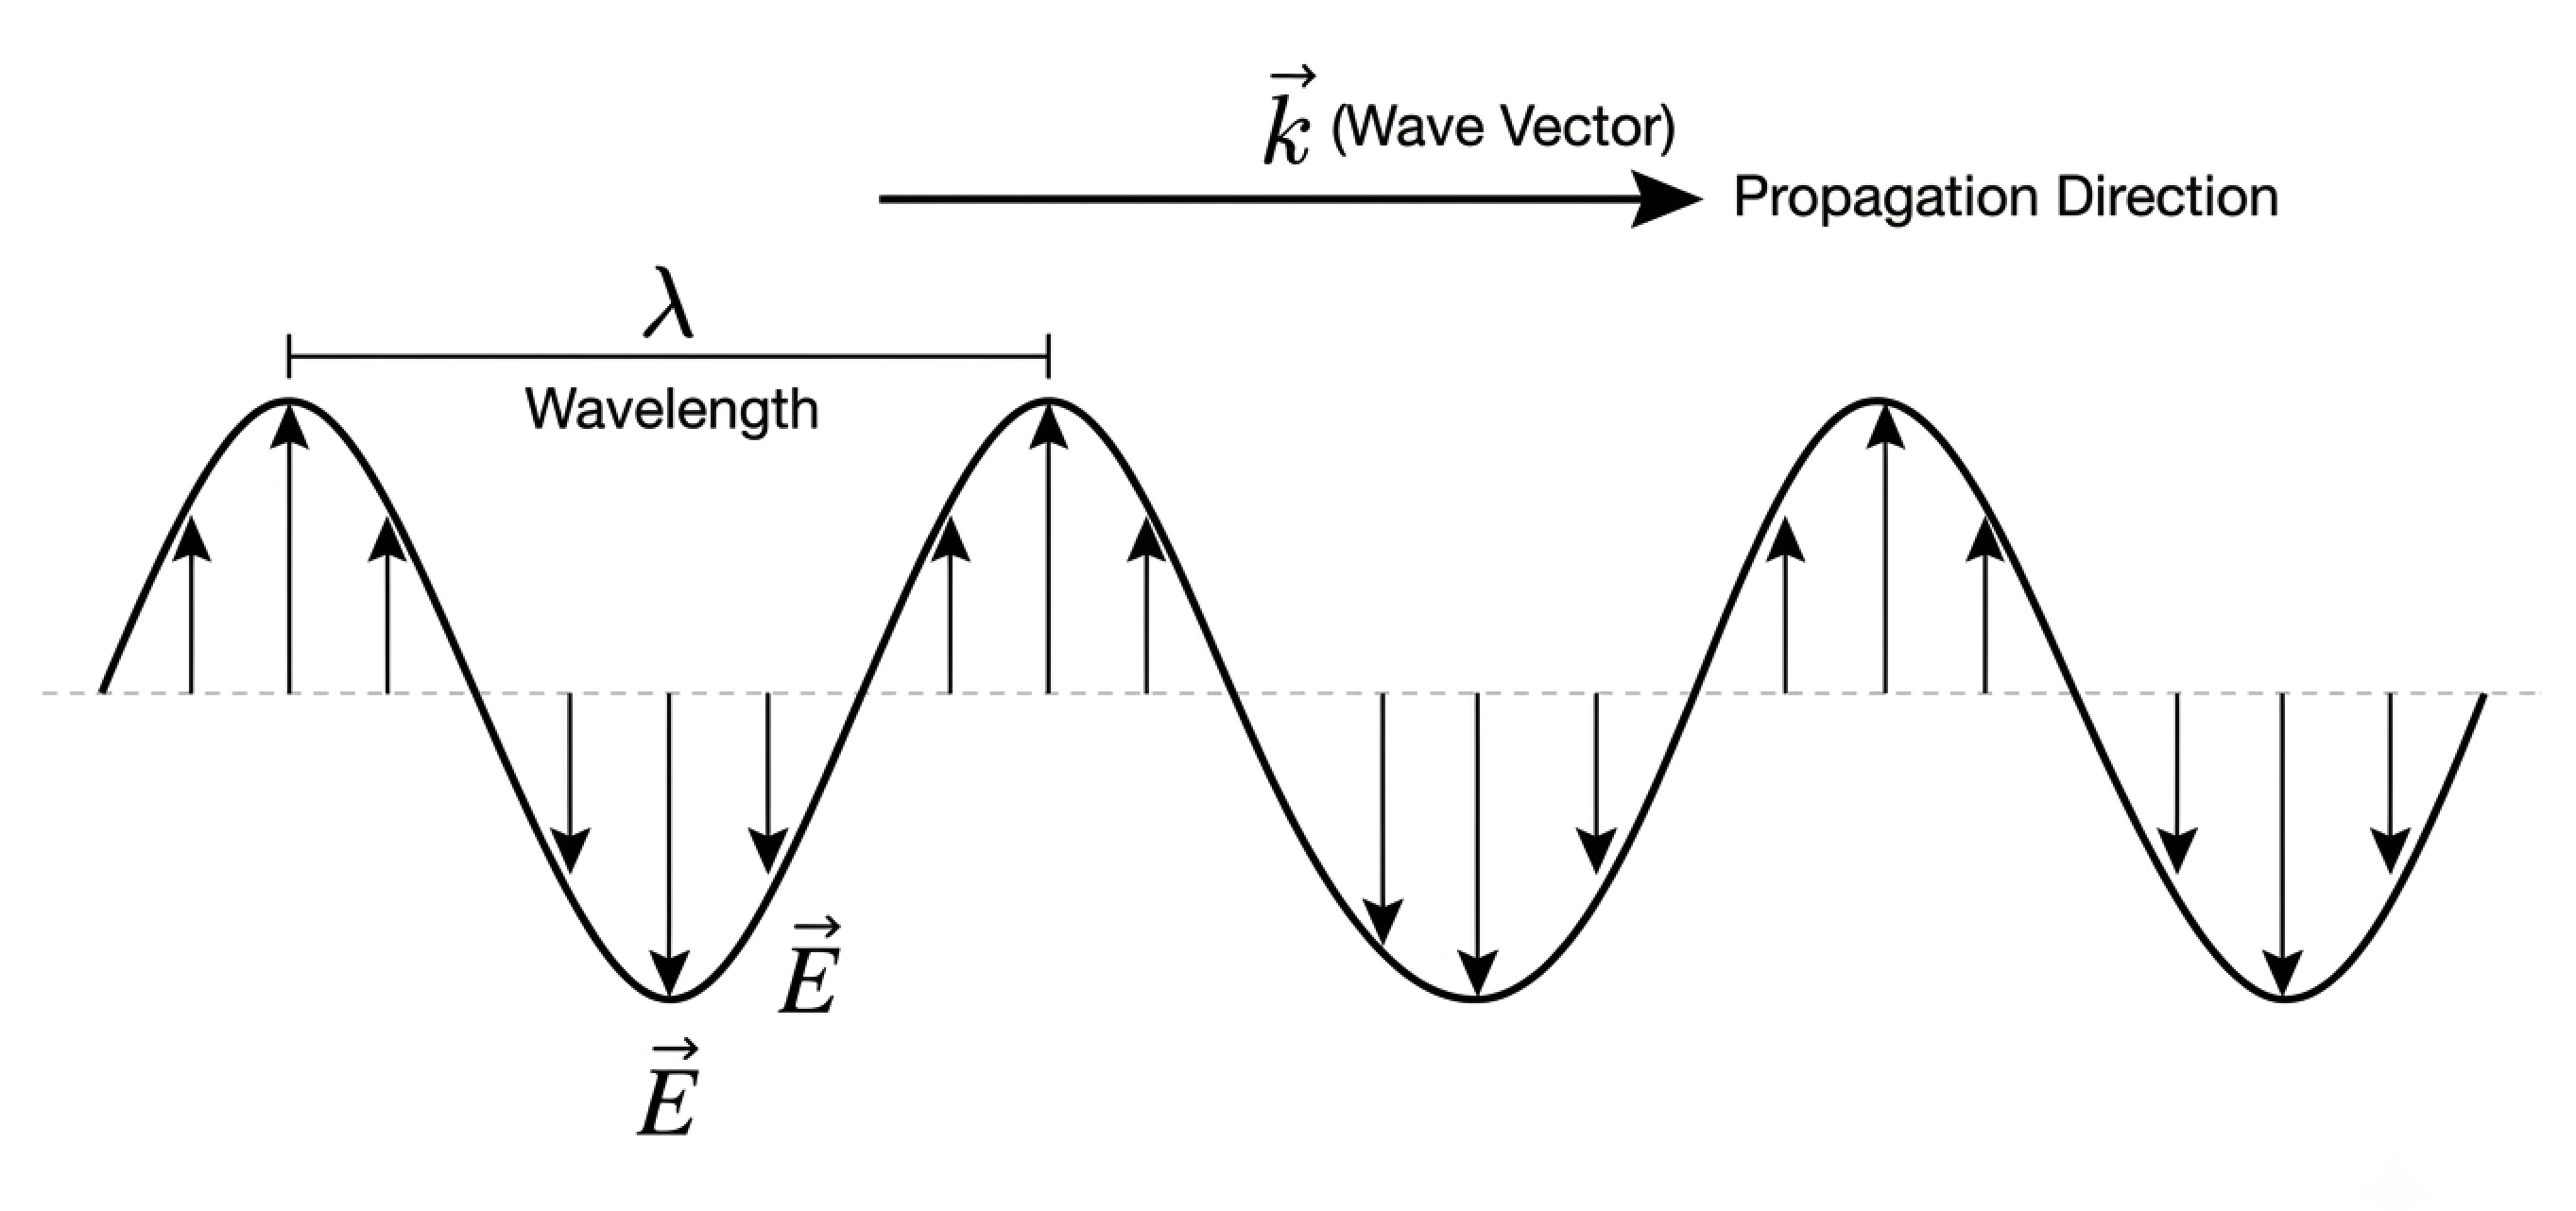
\includegraphics[width=7cm]{images/Fig4}
	\caption{Plane waves in two and three dimensions}
\end{figure}

One of the special solutions for wave equation is called a plane wave and its expressed as
\begin{equation}
	\Psi = \Psi_0 e^{i(k \cdot x - \omega t)} = \Psi_0 [ \cos (k \cdot x - \omega t) + i \sin (k \cdot x - \omega t) ]
\end{equation}
where $x$ denotes a position vector of a three-dimensional Cartesian coordinate. By applying de Broglie and Einstein’s relations, this is converted into a matter wave representing a particle:
\begin{equation} \label{eq:8}
	\Psi = \Psi_0 e^{i(\frac{p}{h} \cdot x - \frac{E}{h} t)}, \quad 
	p = \begin{pmatrix} e_1 \; e_2 \; e_3 \end{pmatrix} \begin{pmatrix} p_x \\ p_y \\ p_z \end{pmatrix}
\end{equation}
taking partial differentiation with respect to $x$ we obtain
\begin{equation}
	\frac{\partial \Psi}{\partial x} = \frac{i}{\hbar} p_x \Psi_0 e^{i(\frac{p}{h} \cdot x - \frac{E}{h} t)} = \frac{i}{\hbar} p_x \Psi \quad \Rightarrow \quad
	\frac{\hbar}{i} \frac{\partial \Psi}{\partial x} = p_x \Psi
\end{equation}
Similarly we have
\begin{equation}
	\frac{\hbar}{i} \frac{\partial \Psi}{\partial y} = p_y \Psi \quad \text{and} \quad \frac{\hbar}{i} \frac{\partial \Psi}{\partial z} = p_z \Psi
\end{equation}
Taking partial differentiation once more 
\begin{equation}
	\frac{\partial^2 \Psi}{\partial x^2} = (\frac{i}{\hbar} p_x)^2 \Psi_0 e^{i(\frac{p}{h} \cdot x - \frac{E}{h} t)} = - \frac{1}{\hbar^2} p_x^2 \Psi \quad \Rightarrow \quad
	- \hbar^2 \frac{\partial^2 \Psi}{\partial x^2} = p_x^2 \Psi
\end{equation}
Similarly we have
\begin{equation}
	- \hbar^2 \frac{\partial^2 \Psi}{\partial y^2} = p_y^2 \Psi \quad \text{and} \quad - \hbar^2 \frac{\partial^2 \Psi}{\partial z^2} = p_z^2 \Psi
\end{equation}
So if we summing both sides of these 3 equation and then dividing by $2m$ ($m$ is the mass of a particle), we have
\begin{equation} \label{eq:13}
	- \frac{\hbar ^ 2}{2m} \nabla^2 \Psi - \frac{p^2}{2m} \Psi
\end{equation}

Now lets get back to equation (\ref{eq:8}) and this time taking partial differentiation with respect to $t$, we obtain
\begin{equation} \label{eq:14}
	\frac{\partial \Psi }{\partial t} = - \frac{i}{\hbar} E \Psi_0 e^{i(\frac{p}{h} \cdot x - \frac{E}{h} t)} = - \frac{i}{\hbar} E \Psi \quad \Rightarrow \quad 
	i \hbar \frac{\partial}{\partial t} = E \Psi
\end{equation}
If we subtract (\ref{eq:13}) and (\ref{eq:14}) we get
\begin{equation} \label{eq:15}
	i \hbar \frac{\partial \Psi}{\partial t} + \frac{\hbar ^2}{2m} \nabla^2 \Psi = (E - \frac{p^2}{2m}) \Psi
\end{equation}
Comparing these equations we find out that momentum $p$ becomes the operator $ \frac{\hbar}{i} \nabla$ and energy $E$ becomes the operator $ i \hbar \frac{\partial}{\partial t}$. Now if we substituting these operators into the classical energy conservation relation (Total energy = Kinetic energy + Potential energy) we have
\begin{equation}
	E = \frac{p^2}{2m} + V
\end{equation}
So now lets rewrite the equation (\ref{eq:15})
\begin{equation}
	i \hbar \frac{\partial \Psi}{\partial t} + \frac{\hbar ^ 2}{2m} \nabla^2 \Psi = V \Psi \quad \Rightarrow \quad
	(- \frac{\hbar ^ 2}{2m} \nabla^2 + V) \Psi = i \hbar \frac{\partial \Psi}{\partial t}
\end{equation}
This is the Time-Dependent Schrödinger Equation (TDSE), a fundamental equation of quantum mechanics. 

If we defind a following Hamiltonian operator $H$ (the sum of two components, the kinetic energy and the potential energy of a quantum system) as 
\begin{equation}
	H \equiv - \frac{\hbar^2}{2m} \nabla^2 + V 
\end{equation}
Then we have a shorthand representation such that
\begin{equation}
	H \Psi = i \hbar \frac{\partial \Psi}{\partial t}
\end{equation}















\break
\begin{thebibliography}{99}

\end{thebibliography}	
\end{document}
